\PassOptionsToPackage{svgnames}{xcolor}
\documentclass[tikz]{standalone}
\usepackage{tikz}
\usepackage{amsmath}
\usetikzlibrary{positioning}
\usetikzlibrary{math}
\usetikzlibrary{calc}
\usetikzlibrary{shapes.symbols}
\usetikzlibrary{shapes.geometric}
\usetikzlibrary{arrows}
\usetikzlibrary{arrows.meta}
\usetikzlibrary{shapes.multipart}

\begin{document}
    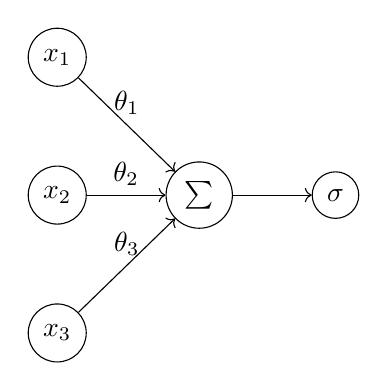
\begin{tikzpicture}[neuron/.style={circle, align=center, draw=black, thin}]
        \node[neuron] (x1) {$x_1$};
        \node[neuron] (x2) [below=of x1] {$x_2$};
        \node[neuron] (x3) [below=of x2] {$x_3$};
        
        \node[neuron] (sum) [right=of x2] {$\sum$};

        \node[neuron] (sigmoid) [right=of sum] {$\sigma$};

        \draw[->] (x1) -- (sum) node[midway, above] {$\theta_1$};
        \draw[->] (x2) -- (sum) node[midway, above] {$\theta_2$}; 
        \draw[->] (x3) -- (sum) node[midway, above] {$\theta_3$};

        \draw[->] (sum) -- (sigmoid);
    \end{tikzpicture}
\end{document}